\documentclass[12pt]{article}
\usepackage[english]{babel}
\usepackage{natbib}
\usepackage{url}
\usepackage[utf8x]{inputenc}
\usepackage{amsmath}
\usepackage{graphicx}
\usepackage{subcaption}
\graphicspath{{images/}}
\usepackage{parskip}
\usepackage{fancyhdr}
\usepackage{vmargin}
\setmarginsrb{3 cm}{2.5 cm}{3 cm}{2.5 cm}{1 cm}{1.5 cm}{1 cm}{1.5 cm}

\title{CT Quality Assurance}					% Title
\author{U.G.C.Jayasankha}								% Author
\date{April 27, 2020}											% Date

\makeatletter
\let\thetitle\@title
\let\theauthor\@author
\let\thedate\@date
\makeatother

\pagestyle{fancy}
\fancyhf{}
\rhead{\theauthor}
\lhead{\thetitle}
%\chead{170259P}
\cfoot{\thepage}

\begin{document}

%%%%%%%%%%%%%%%%%%%%%%%%%%%%%%%%%%%%%%%%%%%%%%%%%%%%%%%%%%%%%%%%%%%%%%%%%%%%%%%%%%%%%%%%%

\begin{titlepage}
	\centering
    \vspace*{0.5 cm}
    
\includegraphics[scale = 0.8]{University_of_Moratuwa_logo.png}\\[1.0 cm]	% University Logo
    \textsc{\Large Department of Electronics and Telecommunication Engineering}\\[0.8 cm]
    %\textsc{\Large University of Moratuwa}\\[1.0 cm]	% University Name
	\textsc{\large BM 3121}\\[0.5 cm]				% Course Code
	\textsc{\Large Medical Imaging}\\[0.5 cm]				% Course Name
	\rule{\linewidth}{0.2 mm} \\[0.4 cm]
	{ \huge \bfseries \thetitle}\\
	\rule{\linewidth}{0.2 mm} \\[1.5 cm]
	
	\begin{minipage}{0.4\textwidth}
		\begin{flushleft} \large
			\emph{Name:}\\
			\theauthor
			\end{flushleft}
			\end{minipage}~
			\begin{minipage}{0.4\textwidth}
			\begin{flushright} \large
			\emph{Index Number:} \\
			170259P									% Your Student Number
		\end{flushright}
	\end{minipage}\\[2 cm]
	
	{\large \thedate}\\[2 cm]
 
	\vfill
	
\end{titlepage}

%%%%%%%%%%%%%%%%%%%%%%%%%%%%%%%%%%%%%%%%%%%%%%%%%%%%%%%%%%%%%%%%%%%%%%%%%%%%%%%%%%%%%%%%%

\tableofcontents
\pagebreak

%%%%%%%%%%%%%%%%%%%%%%%%%%%%%%%%%%%%%%%%%%%%%%%%%%%%%%%%%%%%%%%%%%%%%%%%%%%%%%%%%%%%%%%%%

\section{Introduction to Computed Tomography}
\subsection{Basics of CT}
A CT scan, or computed tomography scan is a medical imaging procedure that uses computer-processed combinations of many X-ray measurements taken from different angles to produce cross-sectional images of specific areas of a scanned object, allowing the user to see inside the object without cutting.[1] 

\begin{figure}[h!]
  \centering
  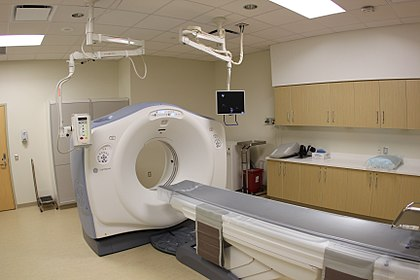
\includegraphics[width=0.45\linewidth]{CT.jpg}
  \caption{\small{X-ray computed tomography (X-ray CT), computerized axial tomography scan (CAT scan)}}
  \label{fig:CT scan}
\end{figure}
As X-ray CT is the most common form of CT in medical applications and various other contexts, the term computed tomography (CT) alone usually refer to X-ray CT, even though other types of tomographic modalities exist such as Positron Emission Tomography (PET) and Single-Photon Emission Computed Tomography (SPECT).

The CT machine consists of a patient support table where the patient is rested for the CT scan and then the area of the patient to be scanned is feed to a doughnut shaped gantry which sends X-rays parallel to the body slice of which the image is taken. The X-ray images thus taken in different angles are fed and stored in a computer system for the reconstruction of the final image. CT can be used to examine various parts of the body such as the chest, abdomen, and pelvic region and also to study organs such as the brain, liver, pancreas, intestines, kidneys, lungs and heart.

CT produces data that can be manipulated in order to demonstrate various bodily structures based on their ability to absorb the X-ray beam. Although, historically, the images generated were in the axial or transverse plane, perpendicular to the long axis of the body, modern scanners allow this volume of data to be reformatted in various planes or even as volumetric (3D) representations of structures. Although most common in medicine, CT is also used in other fields, such as nondestructive materials testing. Another example is archaeological uses such as imaging the contents of sarcophagi or ceramics.
\begin{figure}[h!]
  \centering
  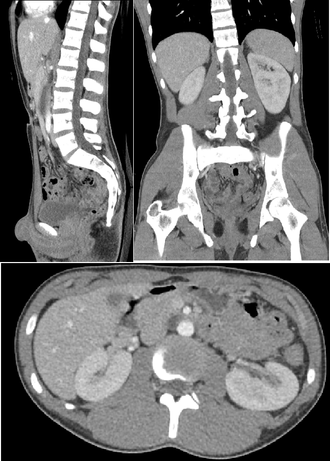
\includegraphics[width=0.45\linewidth]{CT1.png}
  \caption{\small{CT scan of a normal abdomen and pelvis, taken in the axial, coronal and sagittal planes, respectively.}}
  \label{fig:CT scan of a normal abdomen and pelvis, taken in the axial, coronal and sagittal planes, respectively.}
\end{figure}

\subsection{Importance of CT}
Due to several problems and drawbacks of traditional X-ray imaging CT scanning has become superior over it. Computed tomography is engineered to overcome these problems which can not be overcome with traditional projectional x-ray imaging. 
\begin{enumerate}
    \item Low contrast sensitivity\newline
    By observing an traditional x-ray image a 1 cm thick rib or a 1 cm thick air filled trachea can be identified. But anything thinner than that can not be recognized by traditional x-ray imaging. Thus, the blood in the blood vessels, soft tissue details or heart anatomy can not be visible. Possible solution is to inject a liquid contrast medium to blood to make the the contrast enough. \newline

    \item Superposition of 3D structures onto 2D surface
    X-rays are projected through the object and the escaping rays are captured by an X-ray film. Thus images are just 2D projections of 3D objects. The relative distance between objects can not be derived by these images. Furthermore, relative size is not the actual sizes of the objects. 
    \begin{figure}[h!]
        \centering
        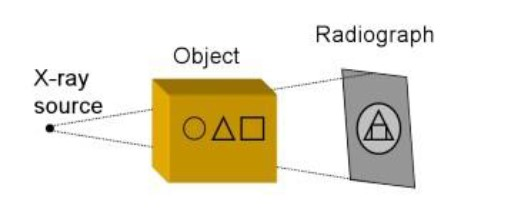
\includegraphics[width=0.65\linewidth]{X1.jpg}
        \caption{\small{Superposition of X-ray}}
        \label{fig:Superposition of X-ray.}
    \end{figure}


    \item Ambiguities with respect to thickness and tissue composition\newline
    X-ray image depicts the x ray intensity at the film after the object. And this is determined according to the attenuation coefficient and the thickness of the object. By observing the image it is impossible recognize wich of the above reasons has been taken part in.
    \begin{figure}[h!]
        \centering
        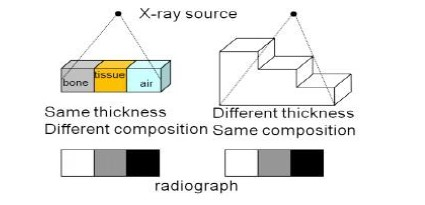
\includegraphics[width=0.65\linewidth]{x2.jpg}
        \caption{\small{Ambiguity of X-ray image}}
        \label{fig:Ambiguity of X-ray image}
    \end{figure}
    
    \newline
    \item Loss of depth information\newline
    As the three-dimensional structure is projected to a two-dimensional image on a film, depth information is lost making it difficult to spatially resolve structures along the direction of X-ray propagation.
    
\end{enumerate}
\pagebreak

\subsection{Components and Implementation of CT}
\begin{figure}[h!]
    \centering
    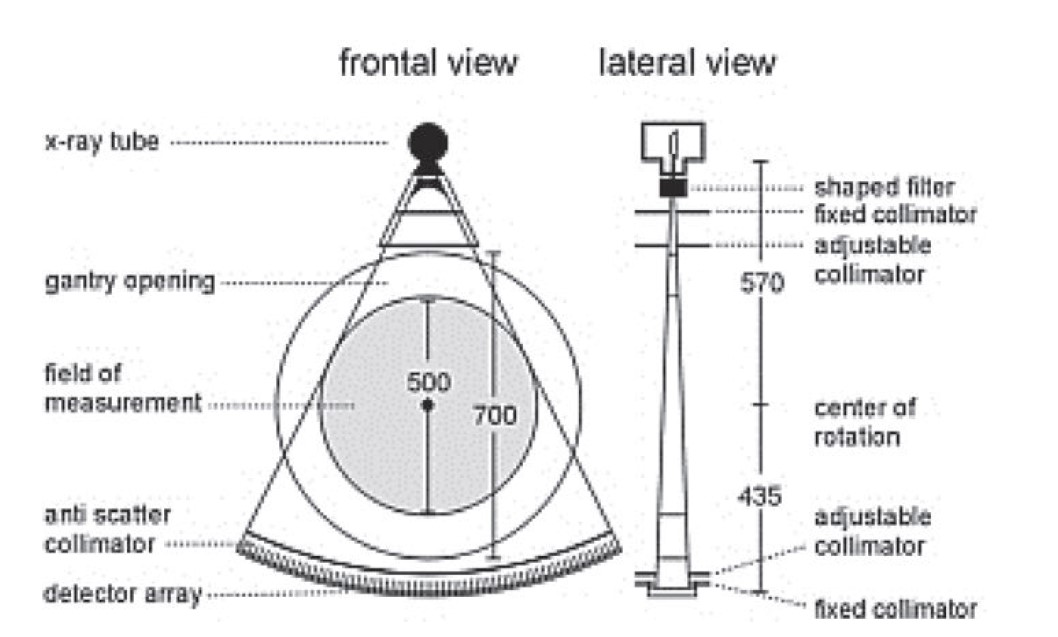
\includegraphics[width=0.85\linewidth]{ct1.jpg}
    \caption{\small{Schematic representation of the scanning geometry and important components of the
CT measurement system in frontal view (x–y plane) and in lateral view (y–z plane).}}
    \label{fig:Schematic representation of the scanning geometry and important components}
\end{figure}

X-ray source is rotating around in the gantry and many attenuation profiles are created in each revolution of the X-ray tube. These profiles are then computer processed and reconstructed to obtain the required cross sectional image.

Components of the CT scanner are,
\begin{enumerate}
    \item Gantry
    \item X-ray generator
    \item Collimator
    \item Filter
    \item Anti-scatter grid
    \item Detectors
    \item Patient couch
    \item Computer system
    
\end{enumerate}

\pagebreak

\section{Quality Assurance Methods of CT}
CT is the most popular imaging modality used to generate 3D to get a clear visualization of the body. When comparing with MRI(the other 3D imaging modality) cost is low, thus more affordable. The quality of the CT imaging system is very important in providing a better health service. The medical diagnosis based on CT imaging depends on the fact that the image is sufficiently suitable to extract required information. Fault analysis is very important for this purpose. Therefore quality assurance must be guaranteed. Otherwise diagnosis will be failed. 
The CT machine consists of many units as mentioned in above topic. Quality assurance of each part or section assures the quality of overall system. 

Furthermore radiation exposure us higher in CT scanning than normal X-ray imaging. Thus it is a serious consequence and must be dealt with extra care. Otherwise The radiation used in CT scanning can lead the patient towards cancers and other genetic diseases. Therefore the need to minimize the radiation exposure of CT imaging is compelling. The usage of multiple X-ray images to construct 3D representation of the image is the primary cause for higher radiation dose in CT. Quality assurance protocols regarding radiation dose is therefore essential to ensure patient safety

To assess the quality of CT systems under the discussed aspects several parameters have been defined and agreed upon by the medical community internationally, regionally or institutionally. Regular tests should be done daily, weekly, monthly, quarterly or annually according to the requirement to identify and correct problems with CT imaging systems.

\subsection{Visual Checklist}
This is the basic method to find flaws in the system and it should be done in every month. Following list of equipment is inspected visually to find any missing part or any malfunction. 

\begin{enumerate}
    \item Correct functioning of table height indicator
    \item Correct functioning of table position indicator
    \item Correct functioning of angulation indicator
    \item Correct functioning of X-ray on indicator
    \item Correct functioning of laser localization light
    \item Smoothness of the table motion
    \item Correct functioning of exposure switch functioning
    \item High-voltage cables are properly attached
    \item Width and the level of the display window is correct
    \item Correct functioning of witches, lights and meters on the panel
    \item Correct functioning of door interlocks
    \item Warning labels are visible
    \item Correct functioning of intercom system
    \item Service records are readily available
\end{enumerate}

If any component fails this list it should be repaired or replaced as soon as possible even before carrying out other quality assurance protocols. 
\newcommand{\mysubscript}[1]{\raisebox{-0.34ex}{\scriptsize#1}}
\subsection{Water CT Number}

CT number is a measurement of the linear attenuation coefficient of a material. CT number is denoted in Hounsfield Unit (HU). The Hounsfield Unit is based on the ratio of the linear attenuation coefficients of water and the material of interests. It is given by,

\begin{equation*}
    HU = \frac{\mu - \mu\mysubscript{Water}}{\mu\mysubscript{Water}-\mu\mysubscript{Air}}
\end{equation*}
\begin{equation*}
    \mu = linear\hspace{0.3 cm} attenuation\hspace{0.3 cm} coefficient\hspace{0.3 cm} of \hspace{0.3 cm}the \hspace{0.3 cm}material
\end{equation*}
\begin{equation*}
    \mu\mysubscript{Water} = linear\hspace{0.3 cm} attenuation\hspace{0.3 cm} coefficient\hspace{0.3 cm} of\hspace{0.3 cm} distilled \hspace{0.3 cm}water\hspace{0.3 cm} at\hspace{0.3 cm} STP   
\end{equation*}
\begin{equation*}
    \mu\mysubscript{Air} = linear \hspace{0.3 cm}attenuation \hspace{0.3 cm}coefficient\hspace{0.3 cm} of \hspace{0.3 cm}air \hspace{0.3 cm}at\hspace{0.3 cm} STP
\end{equation*}

To ensure the constancy of the CT imaging system, it is required to check whether the images obtained by the CT system remains invariant over a period. This is done by imaging a standard object called a phantom and comparing the outcome with the expected outcome. In CT, this is carried out as the measurement of water CT number. A water phantom is usually provided by the equipment manufacturer for this purpose. A CT image is obtained using this phantom as the imaged object. Sample CT slices should be obtained from the middle part of the phantom and the initial or trailing parts. This procedure should be done for both axial and helical canning modes. The settings used for imaging should be the standard CT parameters set for usual clinical imaging parameters.

Two measurements are obtained for this phantom. The mean Hounsfield number of this phantom and the standard deviation. While the mean should ideally be Zero, the variance should satisfy the boundaries set by the manufacturer. However, the limits can be set by the clinical engineer based on the conditions under which the image is obtained, in the case that custom setting were used for the imaging other than the standard prescribed by the manufacturer. Typically the mean should satisfy the following limits for the CT system to be evaluated as normally functioning.

\begin{equation*}
    mean = 0 \pm 3  \hspace{0.3 cm} HU
\end{equation*}

However, irrespective of the settings used the absolute maximum deviation of the mean that is tolerable is ±5 \textit{HU}. The Standard deviation of the Hounsfield Number corresponds to the noisiness of the imaging system. Therefore this corresponds to the radiation dosage used and thus the limits should be decided by the clinical engineer performing the test based on the scan technique. If he chooses to use the limits provided by the manufacturer, he should obtain the phantom image according to the manufacturer’s recommended scan techniques (reconstructed image thickness and filters used for reconstruction). Instead of water phantoms various other standard CT phantoms can be used to evaluate the constancy of the imaging system. However, the limits of acceptability should be obtained from the standards for the phantom used. Usually if mean and variance values fall outside the recommended limits for 3 consecutive tests performed within a week, the constancy of the system is considered to be lost. If the measures indicate that there is some loss of constancy, further tests must be done to isolate the cause of the problem and repairs or replacements should be done.

\subsection{Review of Clinical Protocols}

In every imaging modality there are several specified guidelines to obey when using the system. Those are the clinical protocols of the system. But those procedures may differ according to the patient. To keep the procedures constant over a period of time the parameters, settings and conditions used for imaging for each type of patient and image requirements is reviewed and agreed upon. This protocol is strictly followed in order to avoid mistakes and inconsistencies.

In every imaging system following protocols are used for imaging,
\begin{itemize}
    \item Pediatric head CT (1 year old)
    \item Pediatric abdominal CT (5 years ; 20 kg)
    \item Adult head CT
    \item Adult abdomen CT (about 70 kg)
    \item High-resolution chest CT
    \item Brain perfusion CT
\end{itemize}

There is a set for all the parameters involved in the imaging procedure For each of these CT protocols. Based on the type of image and normally consist of the following special parameters specific for only some protocols must be included as well.

\begin{enumerate}
    \item Tube Voltage - kV
    \item Tube Current - mA
    \item Rotation time
    \item Pitch
    \item Configuration of the detector
    \item Reconstructed image thickness
    \item Reconstruction algorithm or kernels
    \item Breath-hold time
    
\end{enumerate}

\textbf{Computed Tomography Dose Index} - \textbf{CTDI} is a measure of the radiation dose that is emitted from the CT source. While this is not a measure of the radiation dose that is received by a patient under scanning, it is considered that \textbf{CTDI} is a better measurement in regulation and quality control of the radiation. The reason for this is the impractical nature of measuring the actual radiation dose received by the patient during scanning. In reviewing protocols it is necessary to make sure that the \textbf{CTDI} values are in accordance with the recommended values. \textbf{CTDI} can be evaluated both before imaging patient using the CT displayed parameters and after image acquisition based on the recorded images.

\subsection{Rules and Regulations}

There are rules and regulations for the for radiologists and medical practitioners including medical engineers. Following are few examples for such rules and regualtions,

\begin{itemize}
    \item Reconstructed image thickness of standard adult head and abdomen CT should be less than 5 mm.
    \item Minimum possible rotation time for pediatric abdomen should be chosen
    \item Maximum value of detector configuration or beam collimation should be used whenever practical, to improve dose efficiency. Here beam collimation is expressed as NT defined by,
    \begin{equation*}
        NT = N \times T
    \end{equation*}
    With N is the number of X ray channels and T is the thickness of one channel. For example, 4 × 5 mm collimation is up to 30\% more dose efficient than 2 × 5 mm collimation in axial mode with no loss in image quality.
    \item Lower kV settings should be used for pediatric scans and scans that use oral or intravenous contrast agents
    \item High-Resolution Chest (HRC) protocol should sharp filters and should be axial images of thin slices about 10-20 mm apart. If helical images are obtained it should be made sure that diagnostic usefulness is ensured.
    \item Minimum possible dose should be used. The recommended CTDI should never be exceeded for the standard protocols. Radiation dose thresholds should be designed for any custom CT protocol
\end{itemize}

\subsection{Table travel accuracy}
This is a quality assurance method of the x-ray source. This test is use to test the accuracy of the patient table's translational movements. There is a procedure with few steps to conduct this test. If the test fails to prove the accuracy the table need to be repaired. 

Following are the steps,
\begin{enumerate}
    \item Place the special phantom and align the first marker with the axial plane
    \item Add some weight to the table top to simulate it to an actual persons weight
    \item Set the table position indication to zero.
    \item Slide the table to align for the second marker.
    \item Record the position of the table
    \item slide the table to the maximum possible extension and return to the first marker
    \item Record the new position of the table
\end{enumerate}

\pagebreak

\subsection{Dosimetry}
Dosimetry is the measurement of the radiation dose received by the patient during a CT scan. Prior to performing the scan the scanner  provides an calculated Computed Tomography Dose Index (CTDI).

By doing this test it can be verified whether the indicated dose is accurate to the real radiation exposure of the patient. This is need to be done twice in a year to maintain the quality. 

A special phantom with holes is used for this. It is connected to an electrometer that measures the radiation exposure of the chamber along its length. Following figure shows such phantom,
\begin{figure}[h!]
  \centering
  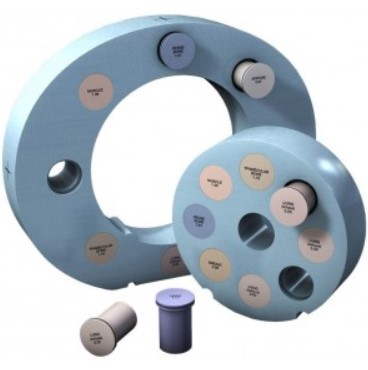
\includegraphics[width=0.45\linewidth]{phantom.jpg}
  \caption{\small{Phantom toolkit for CT}}
  \label{fig:Phantom toolkit for CT}
\end{figure}

\subsection{Alignment Light Accuracy}
Alignment lights are used to check the alignment of the patient. If the alignment is wrong the patient might have to once again. And vulnerable organs of the body can be exposed to radiations. Thus, before doing the imaging, patient is aligned using a light source. A CT phantom with a marker that is opaque to X-rays is placed on the CT table using the alignment light as a guide and the table position is set to zero. A series of images are acquired around this position with about 0.5 mm gap between each slice. Once the obtained images are obtained, the most clearly visible image slices location is found. This distance corresponds to the axial misalignment of the alignment light. If the misalignment is more than 2mm corrective action should be done to restore it to below that limit. 

\subsection{Radiation Beam Width}
Radiation beam width test is used to measure the width of the radiation beam. The optimal value indicated in the scanner differs with the actual width of the X-ray beam. But this gap should be in a safe range otherwise patient is in danger. Therefore this method is used to protect the patient while getting the best results from the imaging

\subsection{Artifact Evaluation}
Artefacts affects the readability of  the image because they would mimic features that are not present in the imaged body. Therefore, artefact evaluation tests must be carried out daily to identify the occurrence of artefacts.

\begin{figure}[h!]
  \centering
  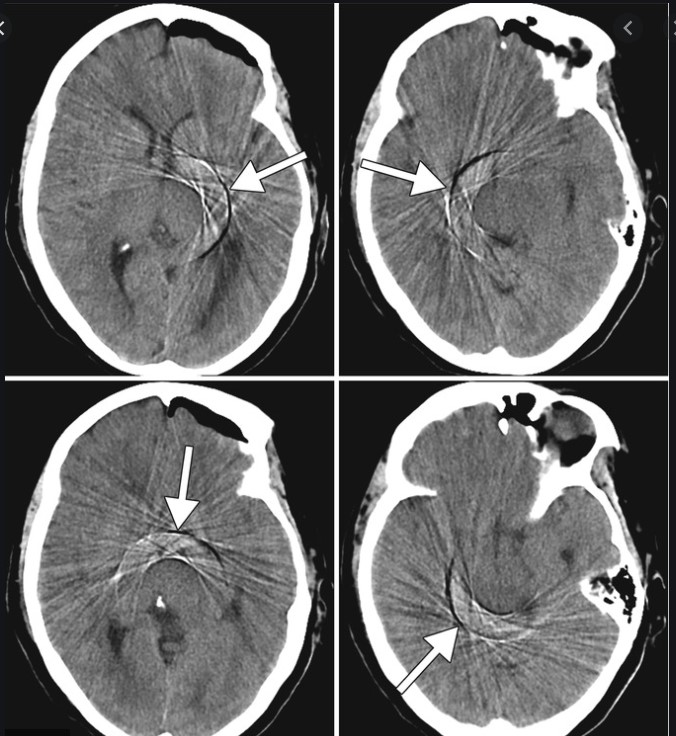
\includegraphics[width=0.75\linewidth]{ar.jpg}
  \caption{\small{Identified artifacts in a CT image}}
  \label{fig:Identified artifacts in a CT image}
\end{figure}

%\subsection{Image Thickness}
\subsection{Spatial Resolution}
This test is performed to verify that the spatial resolution of the CT imaging is sufficient for clinical diagnosis. This test must be done annually or whenever a significant change is done to the system. The following procedure is carried out to evaluate the spatial resolution. 
\begin{enumerate}
    \item The phantom is correctly aligned to the resolution measurement area
    \item Set mA parameters manually to suit the image
    \item Obtain the following scan protocols
    \begin{enumerate}
        \item Adult abdomen
        \item High-resolution chest
    \end{enumerate}
    
    \item Select the image where the contrast indication area is closest to the center
    \item Determine the highest resolution that is visible
(The resolution at which any further increase makes the lines appear as a continuous block)
    \item 6. Select suitable reconstruction algorithm (Sharp reconstruction for chest imaging)
\end{enumerate}

\begin{figure}[h!]
  \centering
  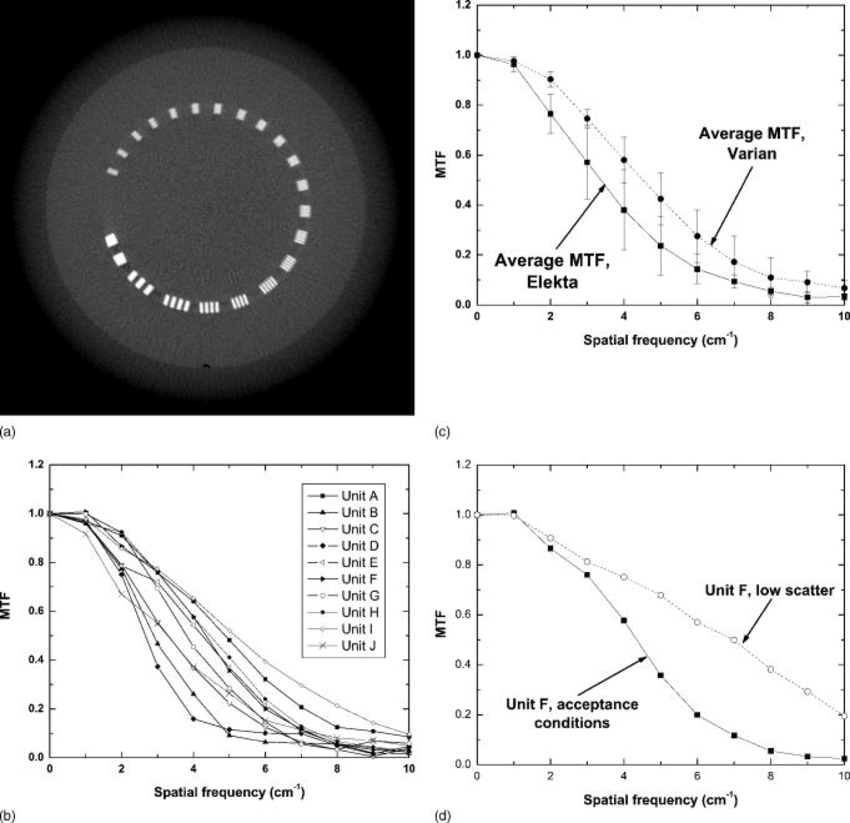
\includegraphics[width=0.55\linewidth]{sr.png}
  \caption{\small{High contrast spatial resolution for seven volumetric imaging systems}}
  \label{fig:High contrast spatial resolution for seven volumetric imaging systems}
\end{figure}

Necessary actions should be taken after checking those values and comparing with the recommended values. 

\subsection{CT number accuracy and Uniformity}
The CT number measured in \textit{Hounsfield} Units is the primary measurement of CT images. Therefore it is required to make sure that the CT number is accurate, Different phantoms with embedded materials with known CT number (Different linear attenuation) are used for this purpose. The test should be performed for several imaging protocols and different \textit{kV} settings annually or after major modifications to the system.

\begin{figure}[h!]
  \centering
  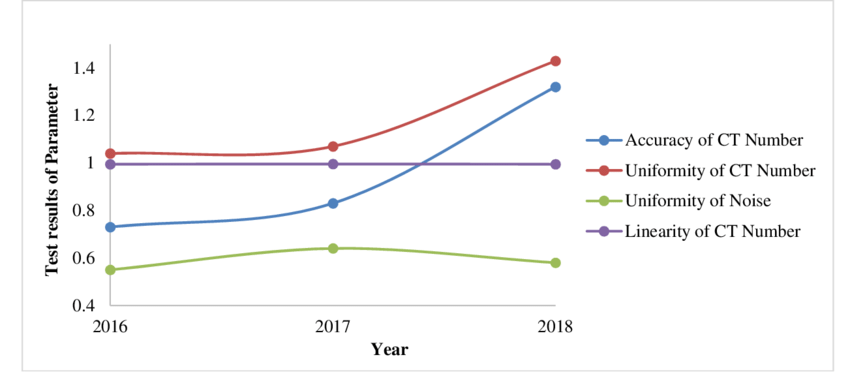
\includegraphics[width=0.75\linewidth]{CTN.png}
  \caption{\small{Parameter variation with time}}
  \label{fig:Parameter variation with time}
\end{figure}
%\subsection{Low Contrast Performance}

\pagebreak
\section{Recent advancements in CT Quality Assurance}
Technology is getting developed within short periods. Therefore there are many additions and updates for the CT systems. Thus CT systems get updated with time. Therefore the old set of quality assurance methods won't work for the new systems. Thus quality assurance methods also should change with the machines. And the system crew members and practitioners should be updated with the new criteria. The solution to these problems is in development of suitable quality assurance protocols to cater for the emerging needs and modifying the existing protocols to suit the needs of the system and the facility. This procedure should be done with extreme care and organization with the involvement of physicians, radiographers, medical physicists, equipment manufacturers and clinical engineers.

\begin{figure}[h!]
  \centering
  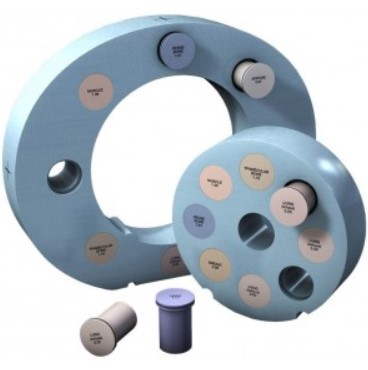
\includegraphics[width=0.45\linewidth]{phantom.jpg}
  \caption{\small{Phantom toolkit for CT}}
  \label{fig:Phantom toolkit for CT}
\end{figure}
\begin{figure}[h!]
  \centering
  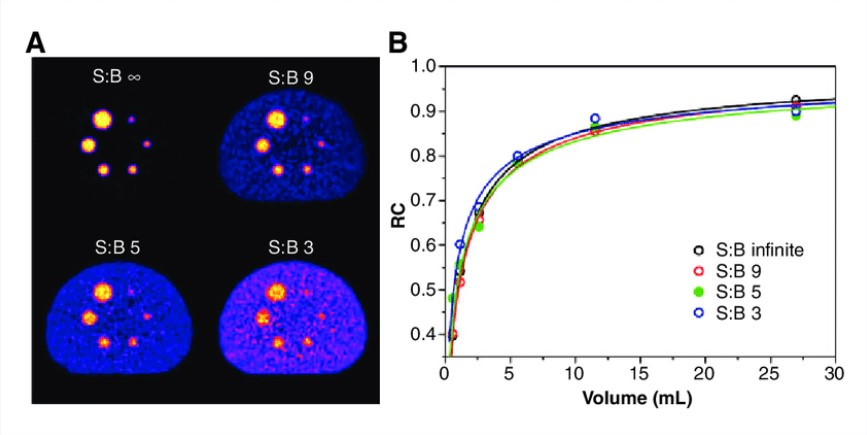
\includegraphics[width=0.65\linewidth]{phantom1.jpg}
  \caption{\small{CT image of a phantom}}
  \label{fig:CT image of a phantom}
\end{figure}

With the advancements in CT systems, advanced QA systems are emerging as well. Instead of having separate tests using separate phantoms, there are recent quality assurance packages that can automatically perform many QA procedures with a single scan. 

Machine learning and data science based approaches have been proposed by many QA analysts and researches to evaluate the correct dosimeter measurements and their effects to internal organs. Since large amount of CT data obtained from different patients with different conditions are available and the availability of powerful computers this might become a possible task.

\pagebreak
\section{Reference}
\begin{enumerate}
    \item International Atomic Energy Agency , "Quality Assurance Program for Computed Tomography," IAEA in Austria, Vienna , 2012.
    \item https://en.wikipedia.org/wiki/CT\_scan
    \item https://www.acr.org/-/media/ACR/NOINDEX/QC-Manuals/CT\_QCManual.pdf
    \item https://www-pub.iaea.org/MTCD/Publications/PDF/Pub1557\_web.pdf
    \item Americal College of Radiology, "Computed Tomography Quality Control Manual," ACR , 2012.
    \item American Association of Physicists in Medicine, "Phantoms for Performance Evaluation and Quality Assurance of CT Scanners," AAPM , 1977.
    
\end{enumerate}
\pagebreak
\textbf{\Large{Appendix}}
\begin{appendix}
  \listoffigures
  %\listoftables
\end{appendix}

\end{document}

